\documentclass[a4paper,12pt]{article} 
\usepackage[T1]{fontenc}              
\usepackage[frenchb]{babel} % césures, titres français
\usepackage[utf8]{inputenc} % encodage
\usepackage[a4paper,left=3cm,right=3cm,top=2cm,bottom=2cm]{geometry} % marges
\usepackage{graphicx} % insertion d'images
\usepackage{rotating}
\usepackage{float} % permet d'utiliser H pour placer un flottant obligatoirement
\usepackage{pdfpages} % inclusion de PDF au sein du document
\usepackage{listings}
\pagestyle{plain} % pied de pages simples

\setlength{\parskip}{1ex plus 0.5ex minus 0.2ex} % espace entre les paragraphes
\setcounter{tocdepth}{2}
\setcounter{secnumdepth}{2}

\lstset{% general command to set parameter(s)
basicstyle=\ttfamily, % print whole listing small
keywordstyle=\color{black}\bfseries\underbar,
% underlined bold black keywords
identifierstyle=, % nothing happens
commentstyle=\color{white}, % white comments
showstringspaces=false,
numbers=left,
language=java,
breaklines=true,
frame=tblr} % no special string spaces

%%%% debut macro %%%%
\makeatletter
\renewcommand\section{\@startsection {section}{1}{\z@}%
                           {-3.5ex \@plus -1ex \@minus -.2ex}%
                           {2.3ex \@plus.2ex}%
                           {\normalfont\Large\bfseries}}
\makeatother
%%%% fin macro %%%%



% Def
\newcommand{\code}[1]{{\lstinline{#1}}}

\begin{document}
\newpage
\title{TP Sécurité des réseaux}
\author{BRIZAI Olivier\\THORAVAL Maxime}
\maketitle

\newpage
\tableofcontents
\newpage


\section{Introduction}
Le but de ce TP est de mettre en place un réseau sécurisé à l'aide d'un firewall CISCO ASA.\\
Ci-dessous, le réseau que nous souhaitons obtenir (les règles de filtrage ne sont pas représentées).

\begin{figure}[H]
	\center
	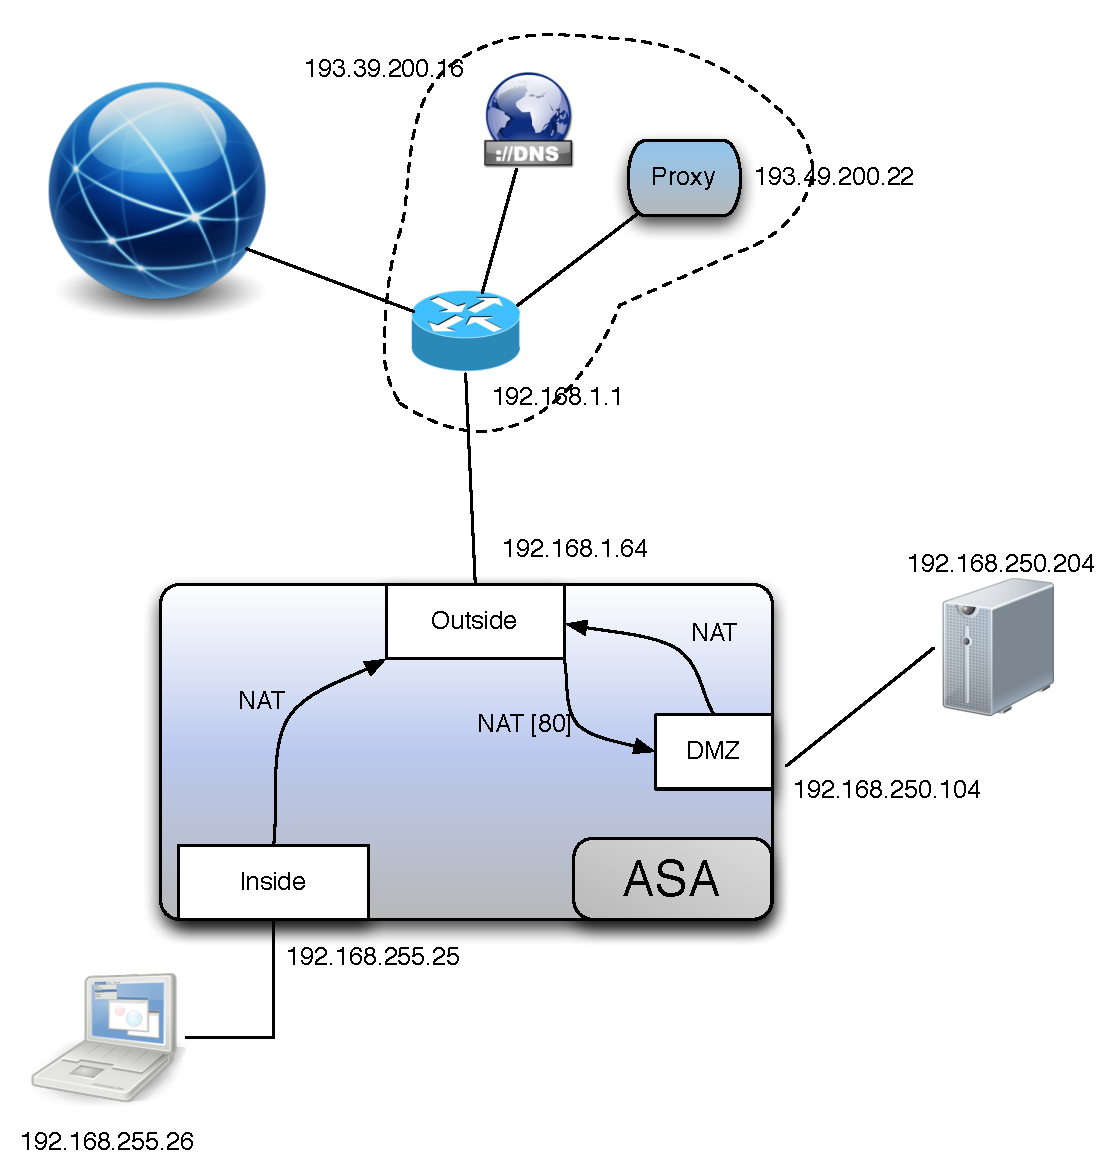
\includegraphics[width=15cm]{img/reseau.pdf}
	\caption{Réseau à obtenir}
\end{figure}

\newpage




\section{Installation et Configurations préliminaires}
\subsection{Client}
Dans un premier temps, nous avons installé Ubuntu 9.04 (version client) sur le PC relié à l'interface \textit{inside}. Ceci effectué, nous réalisons les démarches suivantes, c'est à dire mise en place de Java ainsi que l'installation du paquet \og Minicom \fg.\\
Nous lançons ensuite la commande \textbf{minicom -s} et définissons les divers paramètres afin de configurer le port console. Puis, nous définissons l'adresse \textit{inside} de l'ASA. Nous pouvons maintenant, à partir de celle-ci, accéder à l'interface d'administration de l'ASA au sein de notre navigateur.\\
La figure ci-dessous présente l'accueil de celle-ci. 

\begin{figure}[H]
	\center
	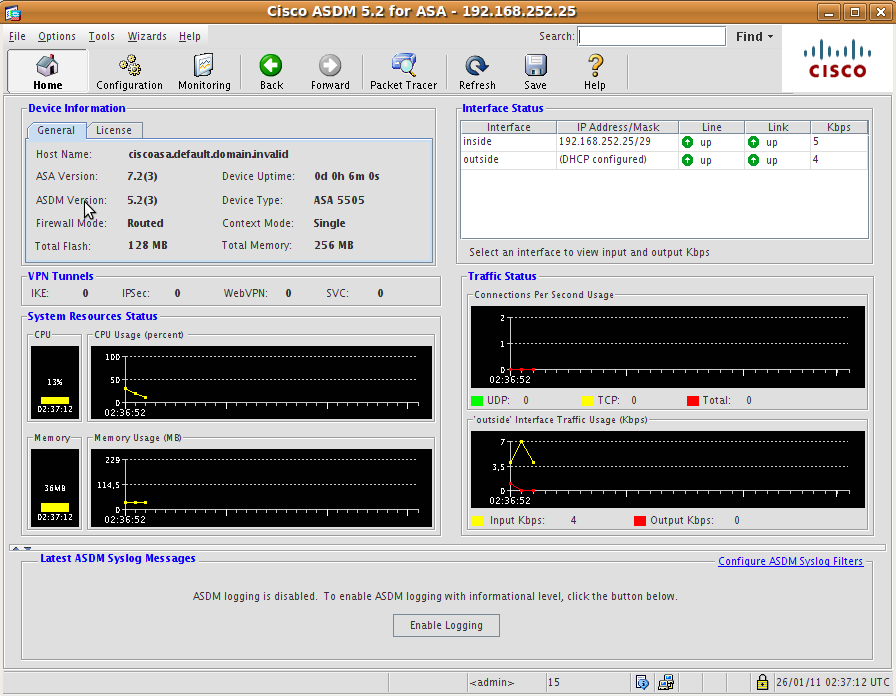
\includegraphics[width=15cm]{img/1-Interfaceconfigfw.png}
	\caption{Interface de configuration}
\end{figure}

Nous avons ensuite utilisé le \og Wizard \fg de l'application pour mettre en place un certain nombres de paramètres tel que adresses IP (inside, outside, dmz) ou encore la répartition des interfaces du firewall (cf. figure ci-dessous). 
\begin{figure}[H]
	\center
	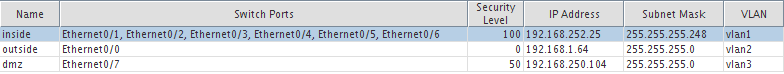
\includegraphics[width=15cm]{img/2-Interfaces.png}
	\caption{Configuration des interfaces}
\end{figure}

Enfin, nous mettons en place une route statique sur l'interface \textit{outside} afin que tous les paquets provenant des autres interfaces soit envoyés par
défaut à la passerelle de l'ENSICAEN.
\begin{figure}[H]
	\center
	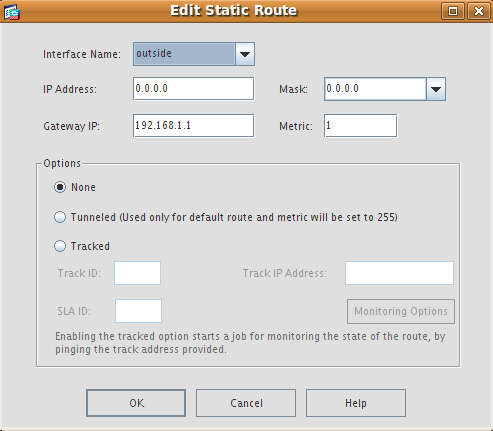
\includegraphics[width=10cm]{img/2-statiqueroute.png}
	\caption{Route statique}
\end{figure}


\subsection{Serveur}
En parallèle, nous installons \og Ubuntu 9.0.4 server \fg{} sur le PC relié à l'interface \textit{dmz} du firewall. Lors de l'installation, nous indiquons que nous souhaitons avoir par défaut les services suivants : un serveur SSH et un serveur web (LAMP).

L'installation terminée, nous allons maintenant configurer les informations réseau de notre serveur. Nous renseignons son adresse IP (192.168.250.204), le masque associé et enfin le routeur (ici il s'agit de l'adresse de l'interface \textit{dmz} de notre firewall).\\
Afin de mettre en place ces informations, nous allons modifier le fichier \textit{/etc/network/interfaces} de la sorte :
\begin{lstlisting}
auto eth0 
iface eth0 inet static
    address 192.168.250.204
    netmask 255.255.255.0
    gateway 192.168.250.104
\end{lstlisting}






\newpage
\section{Configuration Inside}
Dans cette partie, nous avons configuré notre firewall afin de permettre certaines actions au sous réseau relié à l'interface \textit{inside}.

\subsection{Configuration du NAT}
Dans un premier temps, il nous a fallu configurer une règle de NAT afin de traduire l'adresse privée de l'interface \textit{inside} en l'adresse publique de
l'interface \textit{outside}. Nous devons effectuer cette étape afin de réduire les adresses IP utilisées, d'une part dans le but de ralentir la pénurie d'adresse
IPv4, mais aussi pour que la passerelle de l'ENSICAEN n'est qu'une adresse à gérer (celle définie à l'interface \textit{outside}).

Un NAT a pour effet de remplacer les adresses sources des paquets provenant d'un réseau (ou PC) par celle souhaitée (ici remplacement de celles du sous-réseau \textit{inside} par \textit{outside}). Pour les paquets retours (exemple paquet acquitant la réception), le firewall va pouvoir le transmettre
au bon destinataire grâce à une sauvegarde de la transaction.

Ci-dessous, la configuration de notre NAT, pour le sous-réseau de lié à notre interface \textit{inside} (192.168.252.24), nous lions l'adresse de l'interface \textit{outside}.
\begin{figure}[H]
	\center
	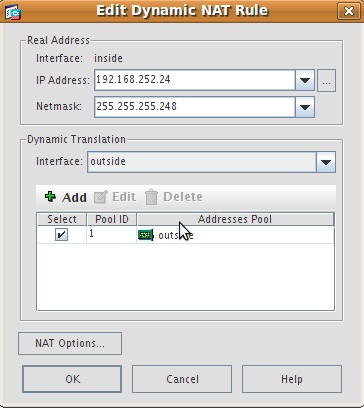
\includegraphics[width=10cm]{img/3-natinsideoutside.png}
	\caption{Configuration du NAT}
\end{figure}


\subsection{Règles de filtrage}
Notre NAT crée, nous allons maintenant mettre en place des règles de filtrage afin de ne laisser passer que les paquets liés à des services définis.
Il faut savoir que lorsque des paquets TCP et UDP sont envoyés, une connexion est établie. Cela permet de n'avoir à définir que les règles de sortie, celles
d'entrées étant liées. Nous pourrons remarquer que le port source des règles est toujours définis sur \og Any \fg{}, en effet, l'application effectuant la demande
n'utilise pas forcément le port dédié.

Chaque règle appliquée ici autorise les services à tout le sous réseau connecté à l'interface \textit{inside}. Il aurait, par exemple, pu être possible de
réduire l'accès au service SSH qu'à certaines machines mais nous pensons que ce n'est pas nécessaire dans le cadre de notre TP.

Dans un premier temps, nous autorisations les flux TCP et UDP sur le port 53 (DOMAIN) qui sont à destination de 193.49.200.16 (adresse du serveur DNS de
l'ENSICAEN).

\begin{figure}[H]
	\center
	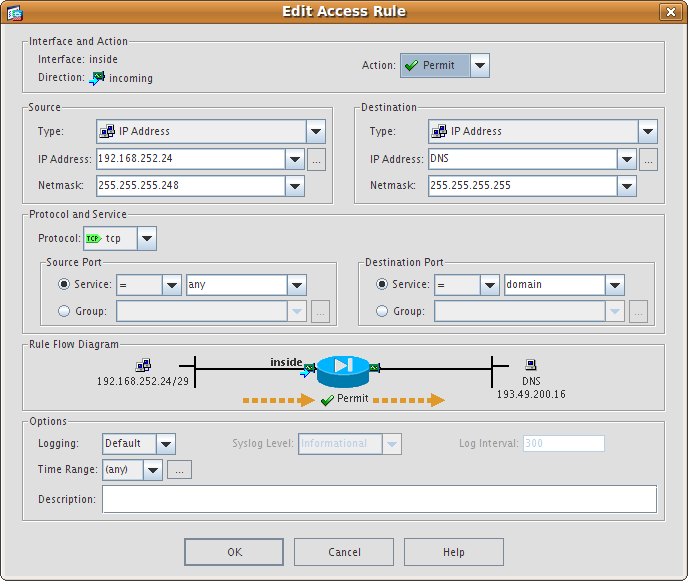
\includegraphics[width=13cm]{img/4-policyinsidednstcp.png}
	\caption{Règle TCP d'accès au DNS}
\end{figure}
\begin{figure}[H]
	\center
	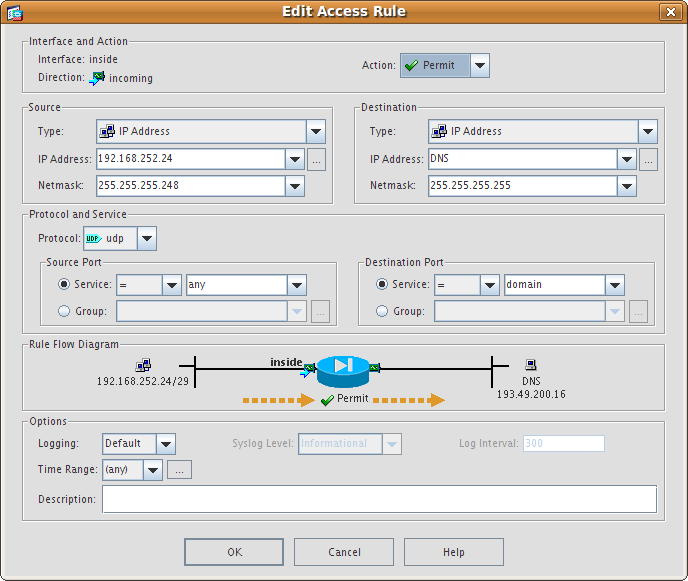
\includegraphics[width=13cm]{img/5-policyinsidednsudp.png}
	\caption{Règle UDP d'accès au DNS}
\end{figure}


\newpage
Maintenant, nous créons la règle autorisant le flux SSH (TCP sur le port 22). Nous ne nous soucions pas de la cible de la demande.
\begin{figure}[H]
	\center
	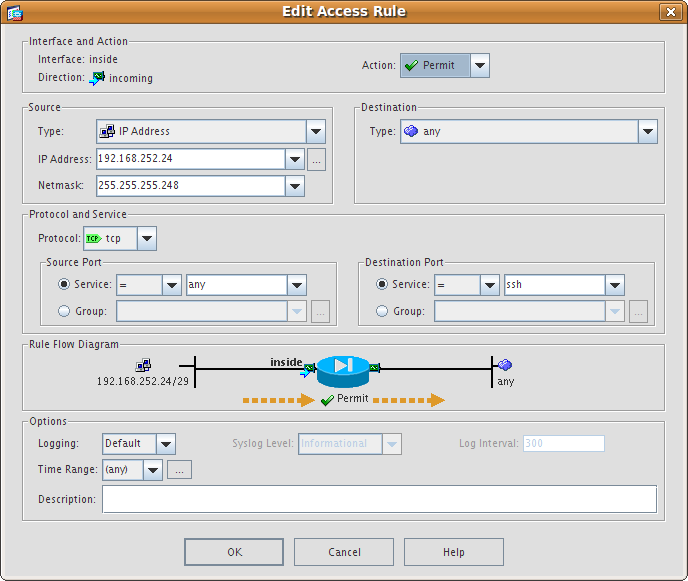
\includegraphics[width=15cm]{img/6-policyinsideanyssh.png}
	\caption{Règle SSH}
\end{figure}


\newpage
Puis la règle autorisant le flux HTTP (TCP sur le port 80) à destination de n'importe quelle machine.
\begin{figure}[H]
	\center
	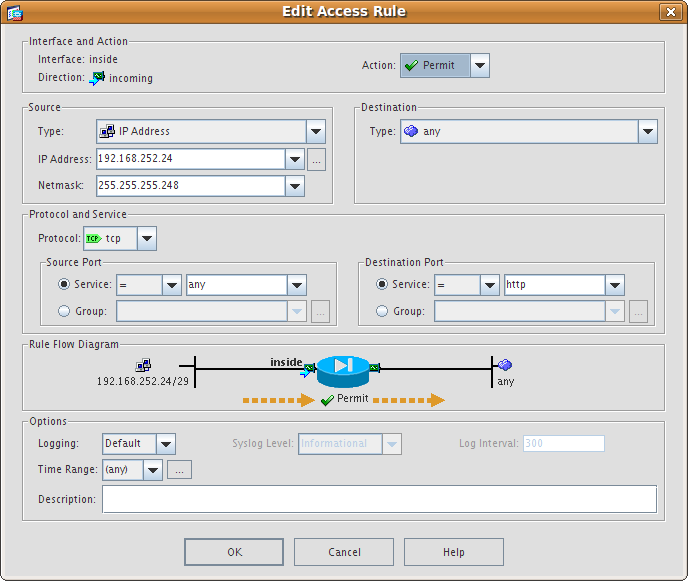
\includegraphics[width=15cm]{img/7-policyinsidehttpany.png}
	\caption{Règle HTTP}
\end{figure}


\newpage
Enfin, nous autorisons le flux à destination d'un proxy (TCP sur le port 3128 = port du proxy de l'école). Bien entendu, nous nous restreignons à l'adresse du
proxy de l'ENSICAEN. 
\begin{figure}[H]
	\center
	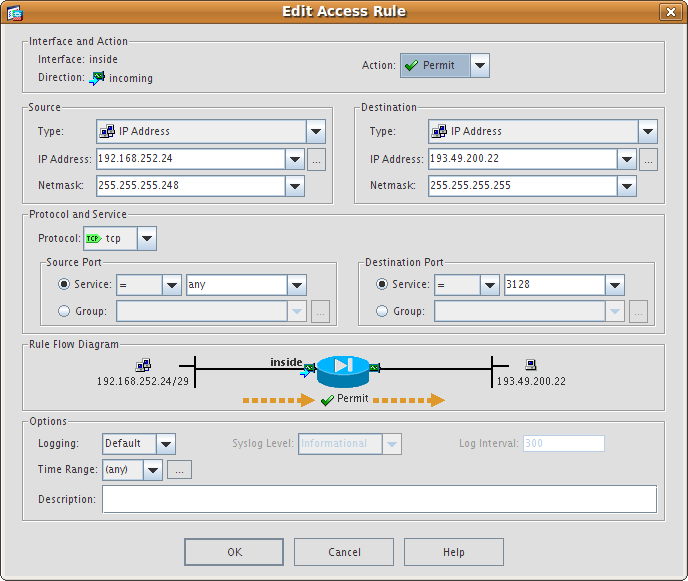
\includegraphics[width=15cm]{img/8-policyinsidetcpproxy.png}
	\caption{Règle Proxy}
\end{figure}


\newpage
\subsubsection{Problèmes rencontrés}
\textit{Ping}

Nous sommes maintenant censé pouvoir accéder au routeur de l'école (adresse 192.168.1.1). Pour le vérifier, nous lançons la commande \textbf{ping} sur son adresse. On remarque que nous n'avons pas de retour de cette commande. Afin de vérifier l'erreur, nous allons regarder le \textit{monitoring} de notre firewall. Ceci va nous permettre de suivre son activité. Après analyse des traces, nous avons pu comprendre l'échec de la commande \textbf{ping}. En effet, elles nous informent que les paquets de type ICMP ne sont pas autorisés à destination de l'interface \textit{inside}. Afin de résoudre ce problème, nous devons rajouter une nouvelle règle de filtrage que nous avons défini de la manière ci-dessous.
\begin{figure}[H]
	\center
	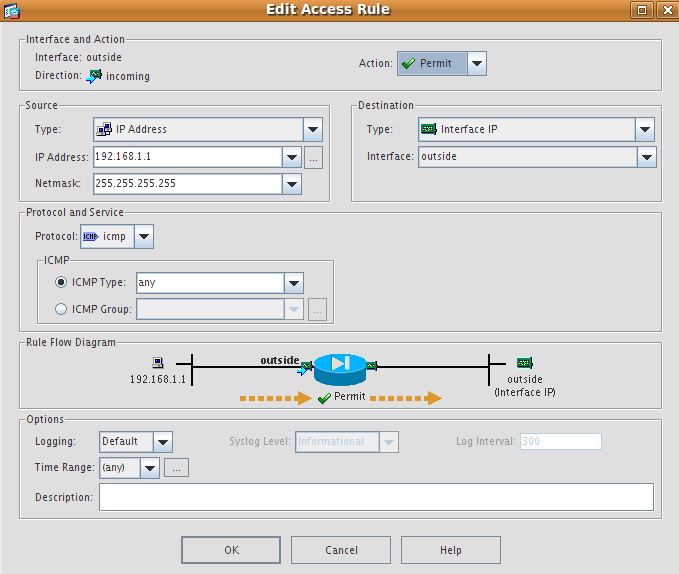
\includegraphics[width=12cm]{img/9-Pingrevientpasflitrageicmp.png}
	\caption{Filtrage ICMP pour autoriser le retour de ping}
\end{figure}

Cette règle mise en place, nous lançons une nouvelle fois la commande \textbf{ping}. Comme visible sur la figure ci-dessous, il n'y a plus d'échec.
\begin{figure}[H]
	\center
	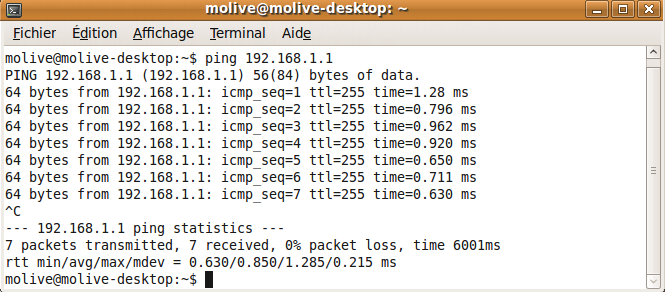
\includegraphics[width=11cm]{img/10-pingok.png}
	\caption{Résultat ping}
\end{figure}

~

\textit{Utilisation du DNS}

La règle du DNS étant active, nous considérions que l'ordinateur branché sur \textit{inside} pouvait accéder à son service. Pour le vérifier, nous avons
essayer plusieurs commandes listées ci-dessous
\begin{lstlisting}
ping google.fr
host google.fr
nslookup google.fr
\end{lstlisting}

Chacune de ses commandes ne fonctionnaient pas, en effet, elles indiquaient qu'elle n'arrivait pas à récupérer l'adresse IP lié au nom de domaine. Etant
donnée que c'est au DNS de nous fournir ces informations, nous avons conclu qu'il y avait un problème de configuration. Pour tester si notre règle de 
filtrage fonctionnait, nous avons effectué ceci
\begin{lstlisting}
	telnet 193.49.200.16 53
	Trying 193.49.200.16...
	Connected to ns.ecole.ensicaen.fr.
	Escape character is '^]'.
\end{lstlisting}

Nous testons la connexion au serveur DNS sur le port 53 (comme définis dans nos règles). Nous remarquons que nous avons pu nous y connecter. (les messages
suivants sont dû au fait que nous utilisions \textbf{telnet} pour nous connecter). Nos règles sont donc fonctionnelles. Afin de vérifier l'utilisation du DNS,
nous avons fait ceci
\begin{lstlisting}
nslookup
> server 193.49.200.16
Default server: 193.49.200.16
Address: 193.49.200.16#53
> google.fr
Server:		193.49.200.16
Address:	193.49.200.16#53

Non-authoritative answer:
Name:	google.fr
Address: 209.85.229.99
Name:	google.fr
Address: 209.85.229.147
Name:	google.fr
Address: 209.85.229.104
\end{lstlisting}

Dans un premier temps, nous indiquons à \textbf{nslookup} l'adresse IP du serveur DNS. Puis, re-testons avec le nom de domaine \textit{google.fr}.
Nous pouvons voir qu'il y a un retour, le DNS est donc utilisable. Après recherche, il se trouve que c'est dans le système Linux en lui-même que 
nous avions oublié d'indiquer l'adresse IP du serveur DNS au moment de rentrer celle de la machine.


\newpage
\newpage
\section{Configuration DMZ}
Maintenant que la configuration du PC client est mis en place et fonctionnelle, nous allons configurer notre serveur. Celui-ci doit être accessible de 
l'extérieur en HTTP et SSH, mais aussi par notre PC client.

\subsection{Configuration du NAT}
Comme pour l'interface \textit{inside}, nous allons définir une NAT afin de traduire les adresses du sous réseau. Etant donné que nous n'avons qu'un serveur
de connecté sur l'interface \textit{dmz}, nous donnons son adresse et non celle du sous réseau.
\begin{figure}[H]
	\center
	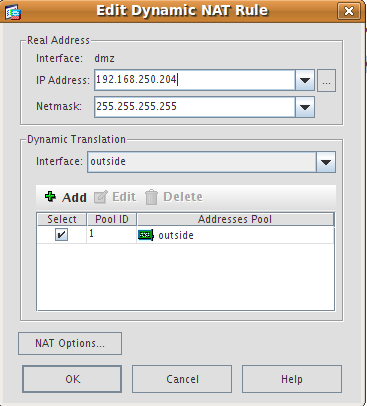
\includegraphics[width=10cm]{img/11-natdmzoutside.png}
	\caption{NAT pour l'interface \textit{dmz}}
\end{figure}

\subsection{Règles de filtrage}
Nous allons aussi autoriser quelques services à notre serveur. Pour toutes nos règles, nous allons limiter l'adresse IP source à celle de notre serveur, en effet,
c'est la seule machine du sous-réseau.

Dans un premier temps, l'accès au serveur DNS. Nous autorisons le flux TCP et UDP sur le port 53 spécifiquement pour notre serveur (192.168.250.204).
\begin{figure}[H]
	\center
	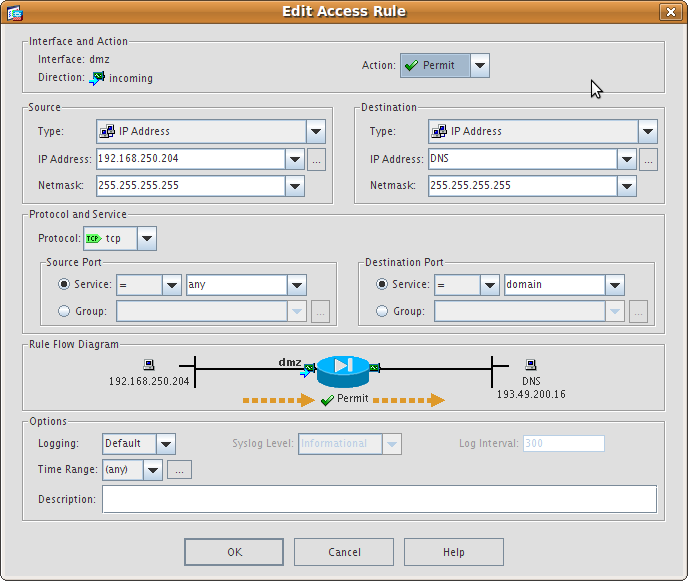
\includegraphics[width=12cm]{img/12-policydmzdnstcp.png}
	\caption{Règle TCP pour l'accès au DNS}
\end{figure}
\begin{figure}[H]
	\center
	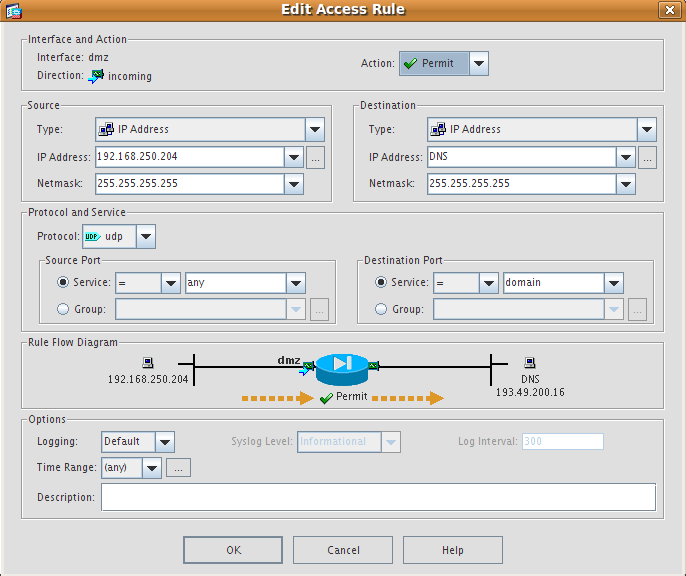
\includegraphics[width=12cm]{img/12-policydmzdnsudp.png}
	\caption{Règle UDP pour l'accès au DNS}
\end{figure}

Nous devons aussi indiquer au système l'adresse du serveur DNS. Pour ce faire, nous éditons le fichier \textit{/etc/resolv.conf} du PC serveur de cette manière.
\begin{lstlisting}
	nameserver 193.49.200.16
\end{lstlisting}

Nous autorisons aussi le flux HTTP et SSH en sortie, tout comme pour l'interface \textit{inside}.
\begin{figure}[H]
	\center
	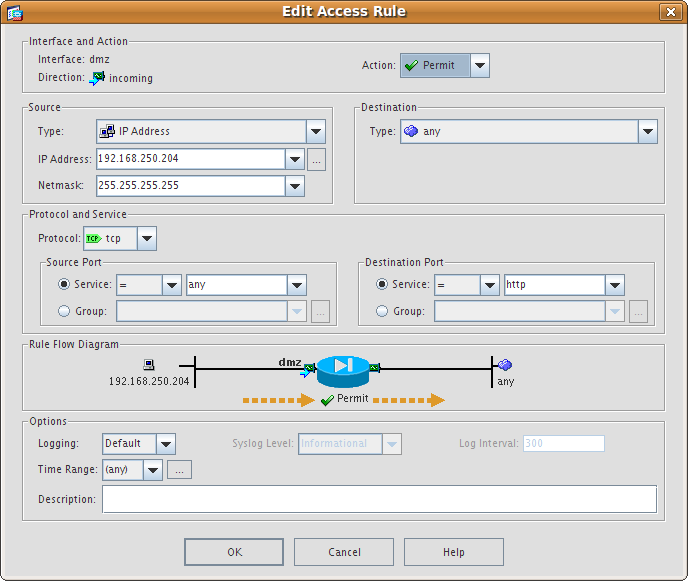
\includegraphics[width=12cm]{img/13-policydmzhttpany.png}
	\caption{Règle HTTP}
\end{figure}
\begin{figure}[H]
	\center
	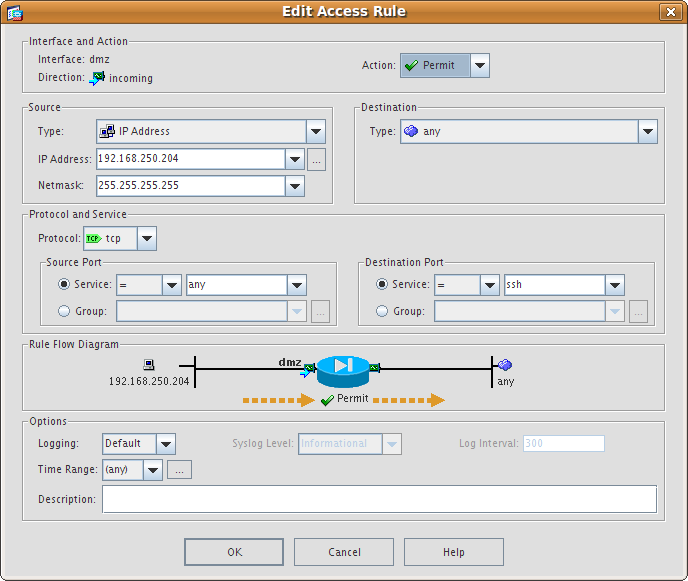
\includegraphics[width=12cm]{img/14-policydmzsshany.png}
	\caption{Règle SSH}
\end{figure}

Nous donnons aussi l'autorisation d'envoyer des paquets en direction du proxy de l'ENSICAEN.
\begin{figure}[H]
	\center
	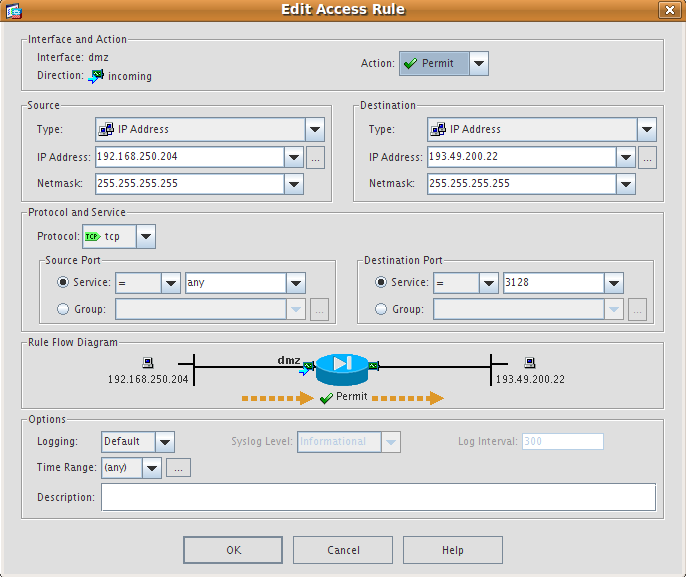
\includegraphics[width=12cm]{img/15-policydmzproxy.png}
	\caption{Règle d'accès au proxy}
\end{figure}

Notre serveur est maintenant capable de discuter avec l'extérieur. Notre but est de pouvoir y accéder à partir de notre client. Pour cela, nous utiliserons 
la technologie SSH. Avant de tester celle-ci, nous allons voir si notre serveur est accessible. Pour cela, nous allons utiliser la commande \textbf{ping}
une nouvelle fois à partir de notre PC client. Nous remarquons que cela ne fonctionne pas, nous ne pouvons y accéder. Les log nous indique qu'il y a un problème
de translation. Ceci est dû au NAT crée entre l'interface \textit{inside} et \textit{outside}. Afin de résoudre ceci, nous allons y créer une exception indiquant
qu'il ne faut pas traduire les messages en provenance du sous-réseau \textit{inside} à destination du serveur (192.168.250.204).

\begin{figure}[H]
	\center
	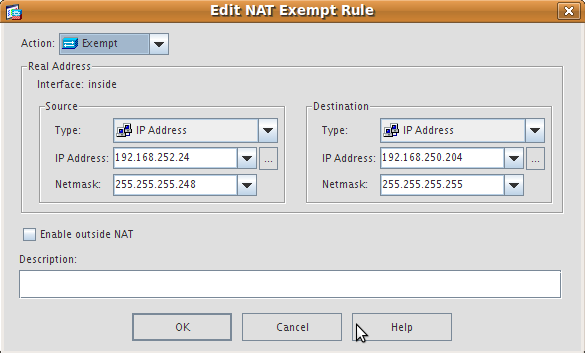
\includegraphics[width=12cm]{img/16-natexception.png}
	\caption{Exception du NAT}
\end{figure}

\subsection{HTTP et SSH à partir du réseau ENSICAEN}
Nous pouvons maintenant accéder à notre serveur à partir de notre PC que ce soit en SSH ou en HTML. Cependant, cet accès est restreint à l'interface
\textit{inside}, en effet, nous souhaiterions que des personnes reliées au serveur de l'ENSICAEN puisse accéder à nos pages web ou encore se connecter en SSH.

Dans un premier temps, nous acceptons les flux HTTP. Nous aurions pu mettre l'adresse IP de notre serveur en tant que destination, mais sachant qu'il n'y a pas
de serveur HTTP sur notre PC client, les utilisateurs n'ont aucun intérêt à aller l'interroger.
\begin{figure}[H]
	\center
	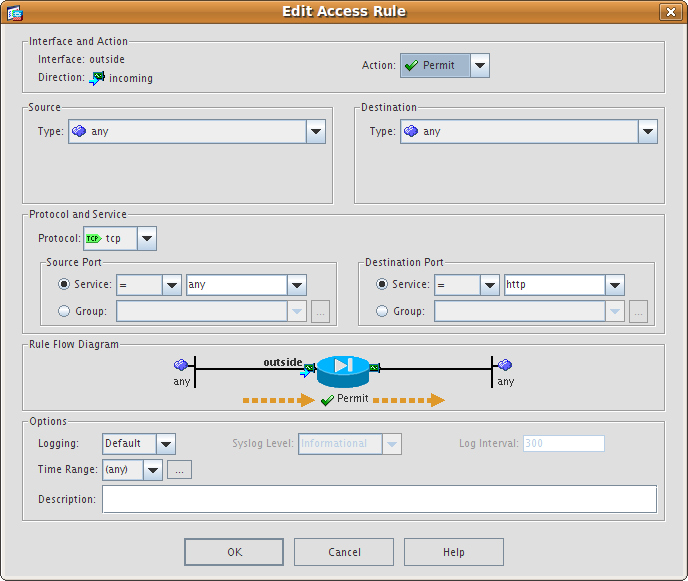
\includegraphics[width=12cm]{img/17-policyoutsidehttpany.png}
	\caption{Filtrage HTTP sur outside}
\end{figure}

Nous configurons maintenant afin qu'il puisse y avoir des demandes de connexion SSH à partir de l'extérieur. Pour plus de sécurité, nous n'avons indiqué que 
l'IP du serveur. Nous aurions aussi pu ne pas le renseigner, limitant l'accès SSH à notre client \textit{inside}.
\begin{figure}[H]
	\center
	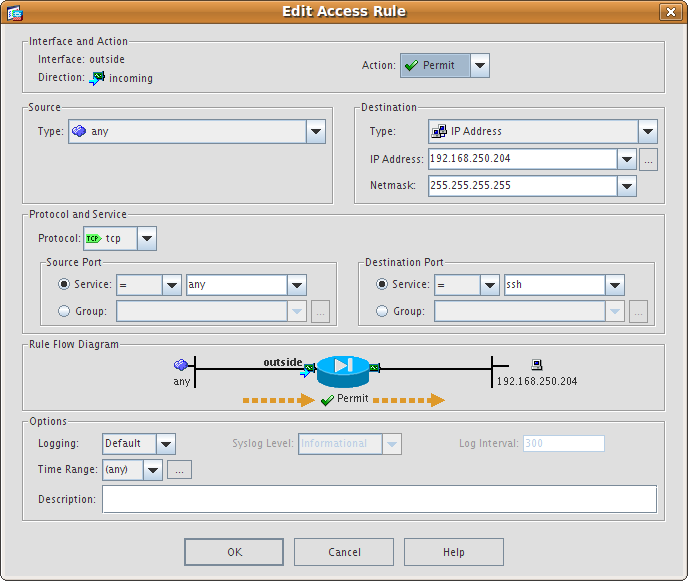
\includegraphics[width=12cm]{img/18-policyoutsidesshserver.png}
	\caption{Filtrage SSH}
\end{figure}

Il nous fallait indiquer au firewall que les flux HTTP et SSH rentrant dans l'interface \textit{dmz} doivent obligatoirement être redirigé à \textit{outside}
en utilisant son adresse. Ci-dessous, les deux NAT statiques définis pour effectuer ceci.
\begin{figure}[H]
	\center
	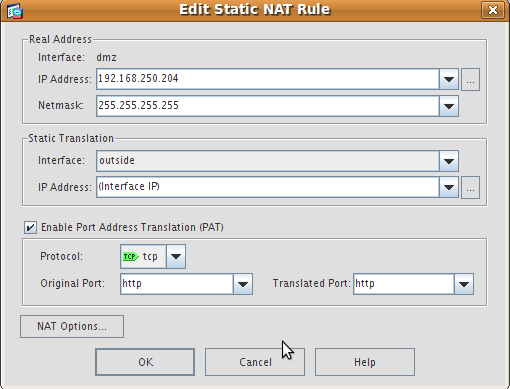
\includegraphics[width=12cm]{img/19-natstaticdmzhttp.png}
	\caption{Route statique pour HTTP}
\end{figure}

\begin{figure}[H]
	\center
	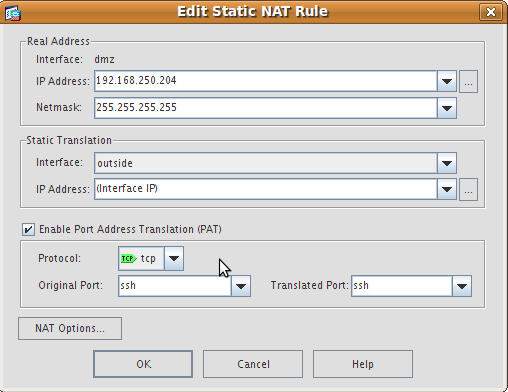
\includegraphics[width=12cm]{img/20-natstaticdmzssh.png}
	\caption{Route statique pour SSH}
\end{figure}

~

A partie de ce moment, il était possible aux personnes présentes dans le réseau ENSICAEN d'accéder à notre serveur HTTP mais aussi à se connecter en SSH.
Vous pourrez trouver en Annexe notre fichier de configuration.

\newpage
\section{VPN}
Suite aux configurations que nous venons d'effectuer, nous avons permis l'accès à notre serveur HTTP et SSH présents dans notre \textit{dmz}.
Cependant, nous souhaitons maintenant permettre l'accès à un serveur de fichier présent sur notre ordinateur relié à la \textit{inside}. Pour ce faire,
nous allons mettre en place une passerelle VPN sur l'ASA.

\begin{figure}[H]
	\center
	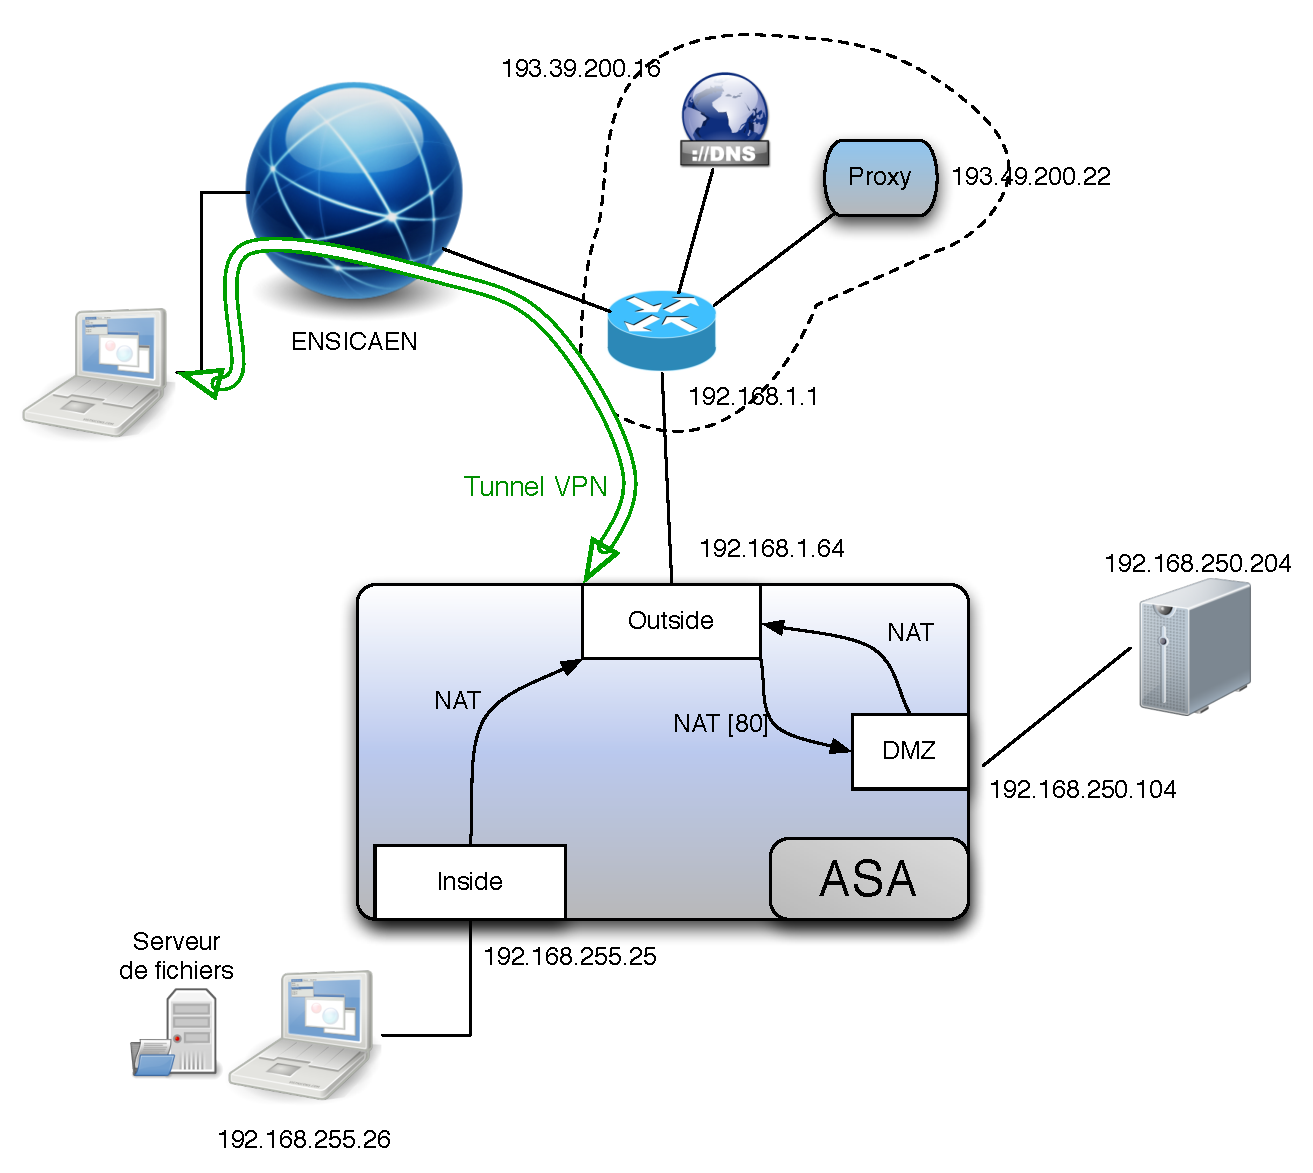
\includegraphics[width=12cm]{img/reseau_VPN.pdf}
	\caption{Architecture du réseau avec mise en place du VPN}
\end{figure}

Afin de sécuriser nos transactions, nous allons utiliser le standard IPsec. N'étant pas forcément géré par tous les clients VPN, nous allons faire que
sa couche soit placée au dessus de UDP (voir ci-dessous).
\begin{figure}[H]
	\center
	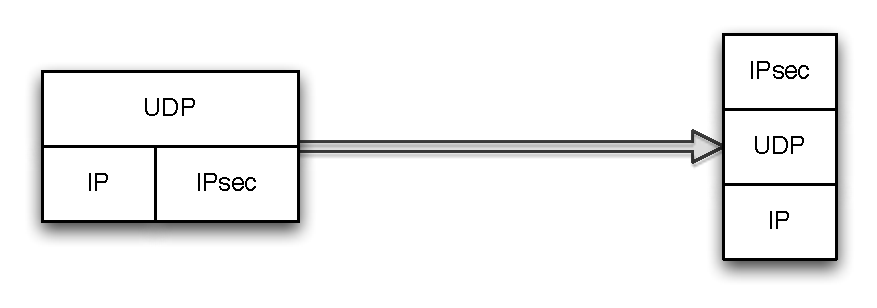
\includegraphics[width=12cm]{img/OSIipsec.pdf}
\end{figure}

\subsection{Présentation}
Le principe du VPN est d'indiquer au PC de l'utilisateur quel chemin prendre pour appeler un serveur cible. Sa mise en place se déroule en plusieurs
étapes : 
\begin{enumerate}
	\item Nous installons le VPN sur notre ASA (configuration détaillée par la suite)
	\item L'utilisateur lance son client VPN et indique les différentes informations (pre\_shared\_key, login, password, ...).
	\item La connexion de l'utilisateur entraîne l'envoie d'informations de la part de l'ASA (adresse IP allouée à la machine, masque, DNS, passerelle, ...).
	\item L'ordinateur de l'utilisateur se charge ensuite de gérer la mise en place du VPN (exemple : simulation d'une nouvelle interface réseau avec 
	modification des routes).
Cela va créer un tunnel entre l'utilisateur et l'ASA. Il va être utilisé spécifiquement lorsqu'il y aura appel au serveur de fichiers.
\end{enumerate}

Une autre information importante indiquant pourquoi nous utilisons IPsec sur UDP et non TCP. IPsec se charge de vérifier si les paquets ont bien été reçus, on dit
qu'il est en mode connecté. TCP effectue les mêmes vérification alors que UDP est en mode déconnecté. Autrement dit, si nous mettons en place IPsec avec TPC, il 
y aurait une double vérification des paquets, ce qui est une perte de temps inutile.

\subsection{Configuration}
Nous allons maintenant configurer notre VPN. Pour cela, nous utilisons le \og VPN Wizard \fg{} de l'interface de l'ASA.

Dans un premier temps, nous renseignons le type de VPN : Remote Access. En effet, c'est un utilisateur distant (hors des interfaces \textit{inside}, 
\textit{dmz} de l'ASA) qui va l'utiliser.
\begin{figure}[H]
	\center
	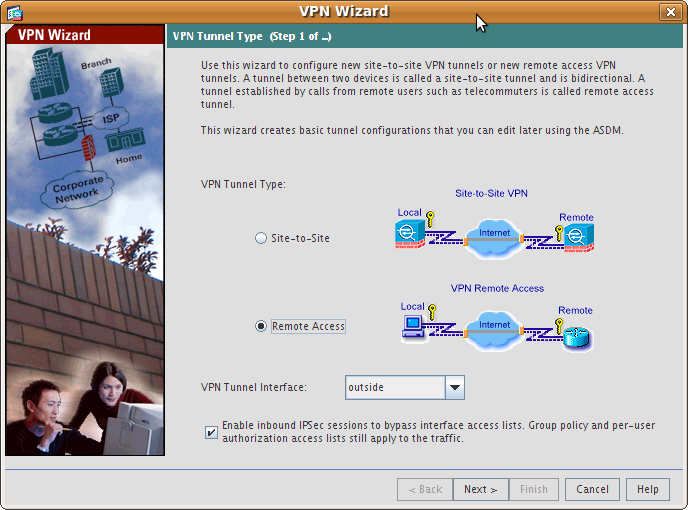
\includegraphics[width=12cm]{img/vpn1.png}
	\caption{Type de VPN}
\end{figure}

Ensuite, nous indiquons le type de logiciel client l'utilisateur va utiliser pour se connecter. Dans notre cas, il s'agit d'un VPN classique.
\begin{figure}[H]
	\center
	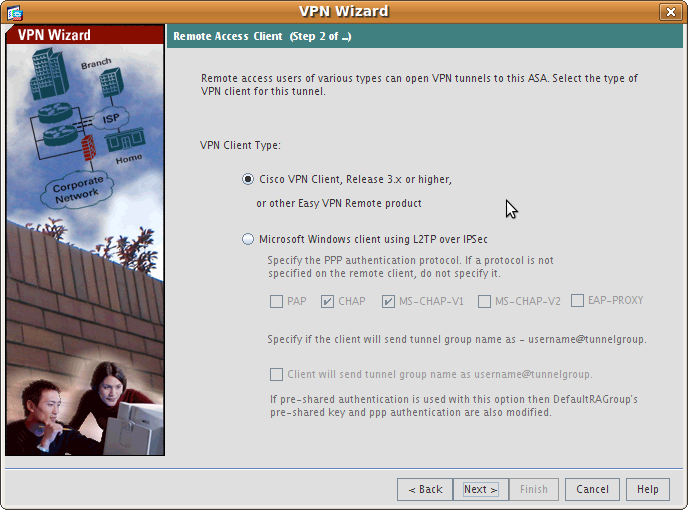
\includegraphics[width=12cm]{img/vpn2.png}
	\caption{Logiciel client}
\end{figure}

Nous configurons maintenant le type d'authentification utilisée. Nous aurions pu utiliser un certificat signé grâce au RSA. Dans notre cas, nous allons
simplement partager un secret (authentification symétrique) qui sera une simple clé : \og tpsecurite \fg. Nous définissons aussi un groupe, ceci permet
de gérer les accès des personnes suivant le groupe auquel ils appartiennent.
\begin{figure}[H]
	\center
	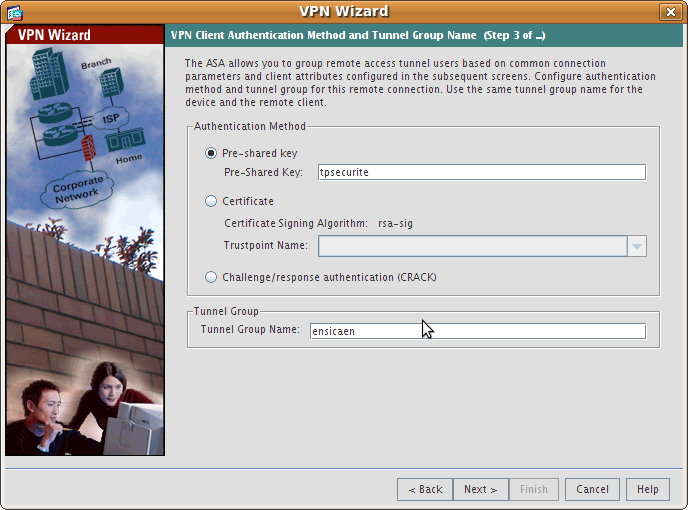
\includegraphics[width=12cm]{img/vpn3.png}
	\caption{Pre\_shared\_key et nom du groupe}
\end{figure}

Nous indiquons à partir de quelle source sont récupérées les données d'authentification du client. Dans notre cas, nous allons les créer au sein de l'ASA.
\begin{figure}[H]
	\center
	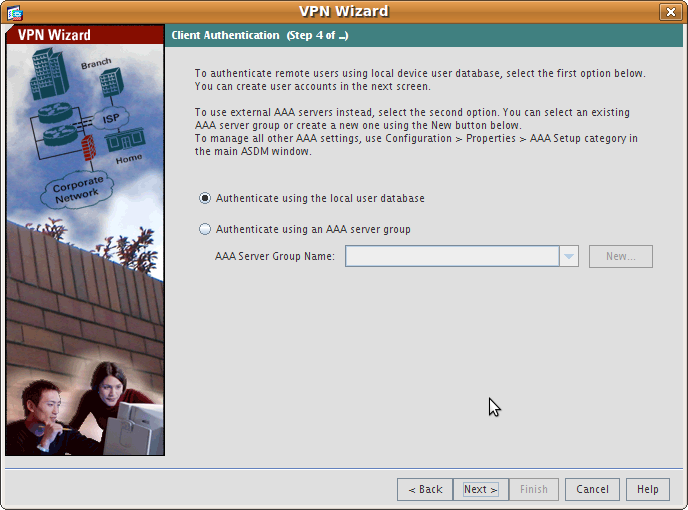
\includegraphics[width=12cm]{img/vpn4.png}
	\caption{Authentification du client}
\end{figure}

Nous ajoutons donc un nouvel utilisateur qui pourra utiliser le VPN. Son login et mot de passe sont simplement \og ensicaen \fg.
\begin{figure}[H]
	\center
	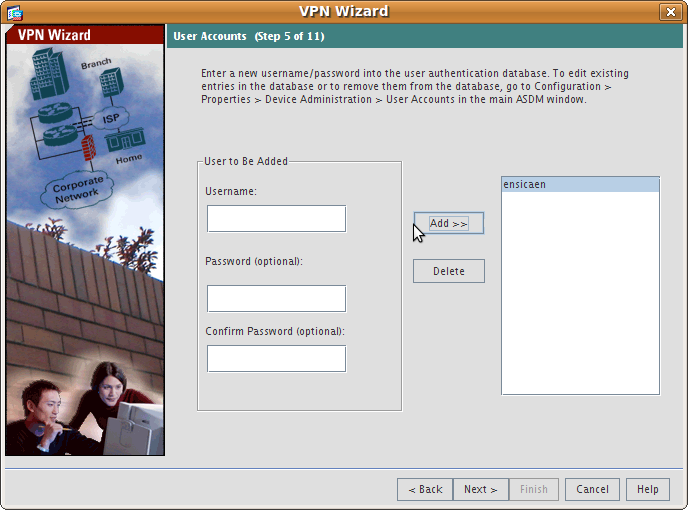
\includegraphics[width=12cm]{img/vpn5.png}
	\caption{Ajout d'un nouvel utilisateur}
\end{figure}

Nous devons aussi définir un pool d'adresses. Il s'agit en fait d'un espace d'adresses à partir duquel l'utilisateur s'en verra attribuer une.
Comme nous n'avons pas encore définis avant, nous allons en créer un. Nous indiquons ainsi que le PC de l'utilisateur pourra se voir octroyer une
adresse entre 192.168.64.1 et 192.168.64.10. Nous pouvons remarquer que le fait de commencer à la première adresse du réseau n'est pas naturel dans le 
monde du réseau. En effet, cette adresse est généralement attribué à la passerelle par défaut.
\begin{figure}[H]
	\center
	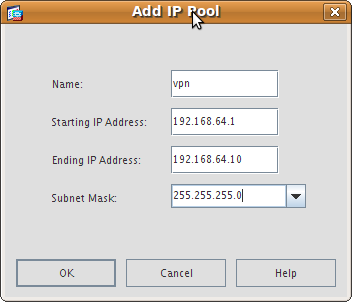
\includegraphics[width=12cm]{img/vpn_pool.png}
	\caption{Pool d'adresses définis}
\end{figure}

Une fois ce pool crée, nous l'attribuons au groupe que nous avons précédemment définis.
\begin{figure}[H]
	\center
	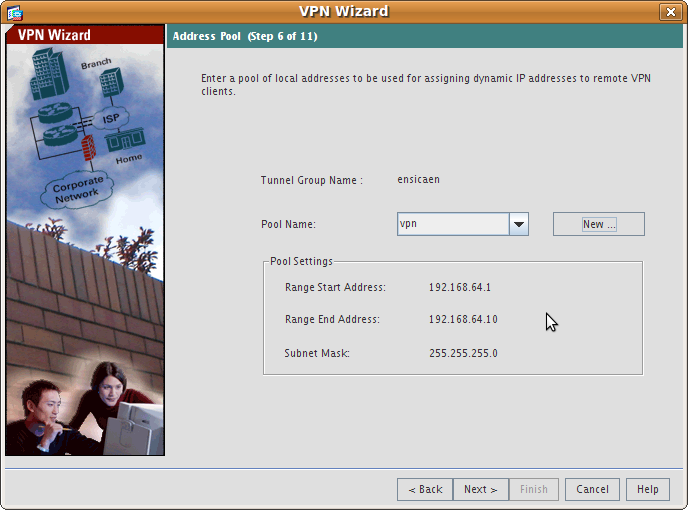
\includegraphics[width=12cm]{img/vpn6.png}
	\caption{Choix du pool d'adresses}
\end{figure}

Nous pouvons définir différentes informations plus ou moins utile suivant le contexte. Celles-ci seront transmises à l'utilisateur que son logiciel client VPN
se chargera de prendre en compte. Dans notre cas, nous allons simplement définir l'adresse du serveur DNS.
\begin{figure}[H]
	\center
	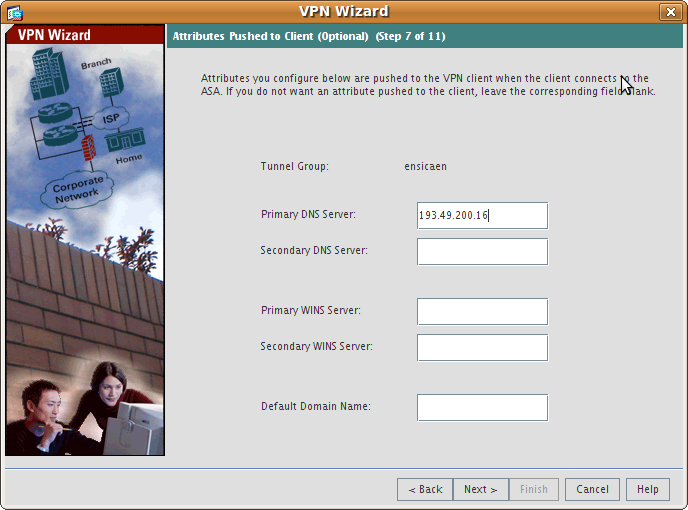
\includegraphics[width=12cm]{img/vpn7.png}
	\caption{Indication du serveur DNS}
\end{figure}

Maintenant que notre VPN est crée, il nous faut indiquer que les paquets reçus par l'utilisateur, connecté en VPN, seront transmis au sous-réseau
relié à l'interface \textit{inside}.
\begin{figure}[H]
	\center
	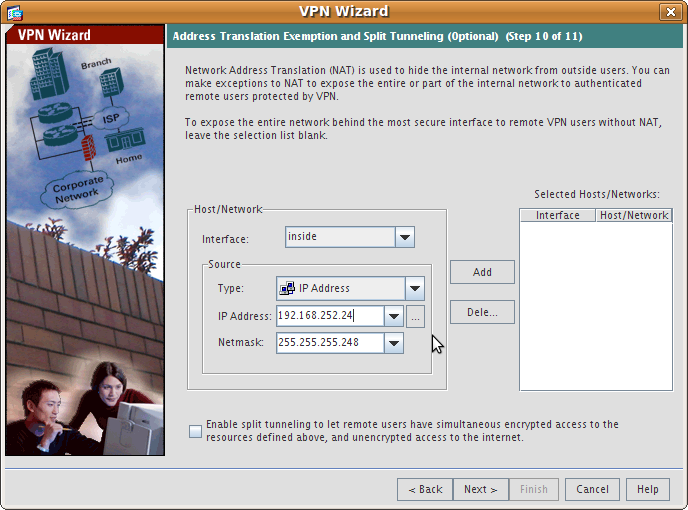
\includegraphics[width=12cm]{img/vpn8.png}
	\caption{Translation d'adresse vers la \textit{inside}}
\end{figure}

Maintenant que la configuration est terminée, nous avons tester à partir d'un ordinateur distant. Il a fallu signaler le mode de fonctionnement
utilisé pour IPsec, ainsi que la clé partagée. Une fois connecté, nous avons pu constater que le logiciel client avait mis en place une interface réseau.
Celle-ci possédait l'adresse 192.168.64.1 et que la passerelle par défaut était 192.168.64.2 (non habituel en réseau). Nous ne pouvions cependant pas
accéder à Internet.

Pour cela, nous avons mis en place une translation d'adresse sur l'interface \textit{dmz} sauf que cette fois, nous autorisons l'utilisateur 
à accéder à Internet de façon non cryptée.
\begin{figure}[H]
	\center
	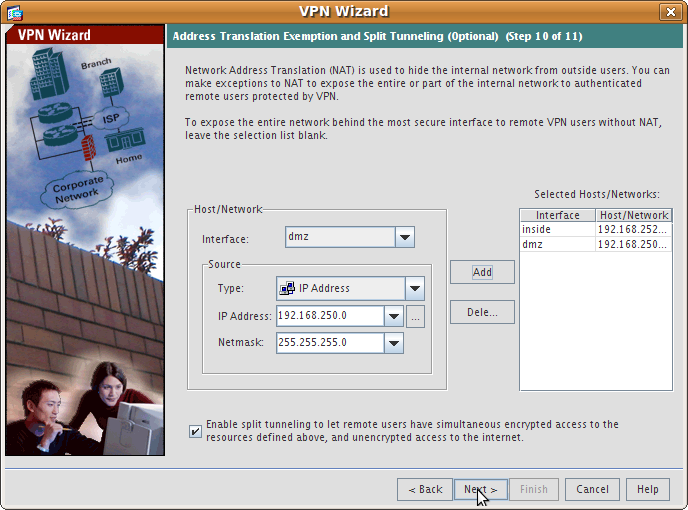
\includegraphics[width=12cm]{img/vpnwizard_alt.png}
	\caption{Translation d'adresse vers la \textit{dmz}}
\end{figure}

Après un nouveau test, cette fois, nous pouvions accéder à Internet. Nous avons pu constater que des routes ont été mises en place afin de définir où
envoyer les paquets à destination de notre sous-réseau \textit{inside}, ainsi qu'à destination de la \textit{dmz}.

\newpage
\section{Outils}
Dans cette section, nous allons voir différents outils permettant de mettre à jour des vulnérabilités du système ainsi que les attaques subis.
N'ayant pas pu tester ces outils à l'ENSICAEN, nous les avons utiliser au sein d'un réseau privé. Tous les tests ont été effectués sous Mac OS X.

\subsection{Wireshark}
C'est un outil performant permettant de sniffer un réseau et d'afficher les paquets émis et reçu sous un format ergonomique. En effet, chaque paquet 
sont affichés et découpés selon les couches ISO avec présentation de nombre d'informations (flag, protocole, checksum, ....). De plus, celui-ci possède 
un outils de filtrage performant. Enfin, il inclut un grand nombre d'outils permettant l'analyse des paquets (encodage d'une conversation audio sur IP, 
possibilité de suivi d'une connexion TCP, ....).

\subsection{nmap}
Il s'agit d'un logiciel d'analyse de ports, services et un informations sur le système d'une ou plusieurs cibles. Il est ainsi possible
de récupérer la liste des ports ouvert (et de ce fait les applications liées) pouvant être la cible de potentielles attaques. Plusieurs scénarios 
d'attaque sont disponibles, exemple attaque de tout un sous réseau afin d'en comprendre son architecture mais aussi d'y découvrir des vulnérabilités.
Pour notre exemple, nous allons dans un premier temps récupérer la liste de tous les ordinateurs de notre réseau à l'aide de la commande ci-dessous :
\begin{lstlisting}
nmap -PN -sL 192.168.1.0/24
-PN : Permet de considerer que toutes les cibles sont en lignes + certaines machines bloquent les pings, cet parametre permet de d'outrepasser cette limite
-sL : Indique que l'on souhaite juste lister toutes les machines du reseau
-192.168.1.0/24 : Reseau a analyser
\end{lstlisting}
Nous récupérons une liste de machines (nom d'hôte) ainsi que leur adresse IP associée.

Nous allons maintenant choisir une cible et essayer d'obtenir plus d'informations. Ci dessous la commande à utiliser ainsi que le résultat de celle-ci.
\begin{figure}[H]
	\center
	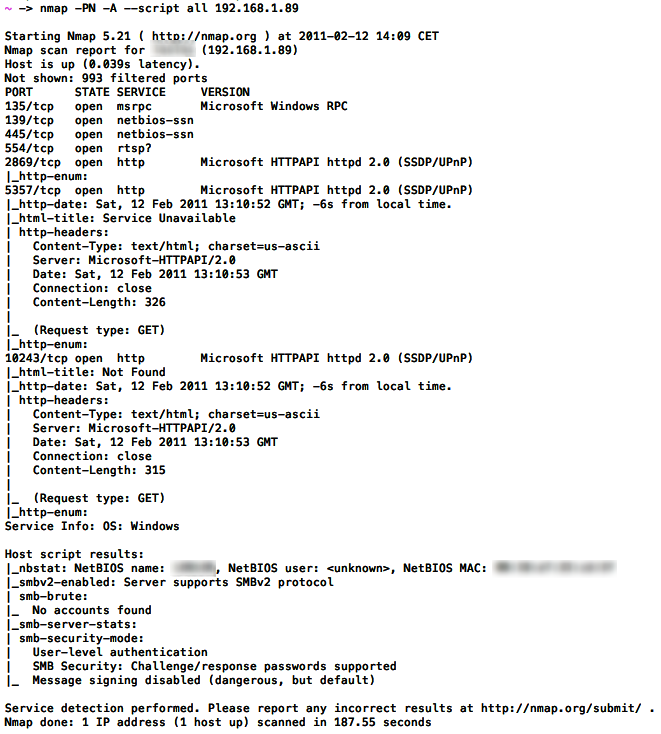
\includegraphics[width=15cm]{img/nmap.png}
	\caption{Commande nmap et résultat}
\end{figure}

\begin{itemize}
	\item -A permet d'afficher des informations sur le système d'exploitation de la cible.
	\item --script all : Indique que nous souhaitons lancer la totalité des scripts sur la cible afin de récupérer un maximum d'informations
	\item 192.168.1.89 : Cible de l'attaque 
\end{itemize}

Pour ce qui est des résultats, dans un premier nous avons des informations sur les ports de la cible. Nous pouvons voir la liste des ports ouverts
ainsi que les applications liées. On peut distinguer plusieurs ports ouverts pour le protocole HTTP, ils sont donc listés avec les entêtes.\\
Ensuite, nous avons des informations sur le service smb (mode de sécurité, compte existant, ...). 

\subsection{Nessus}
Cette application permet de mettre en évidence un certain nombre de failles sur un système. Il fonctionne à l'aide d'un serveur et d'un client.
Nous lançons dans un premier temps le serveur et créons un compte client. Puis, nous lançons le client qui s'y connecte. C'est au sein de se dernier 
que nous pouvons définir un certain nombre de paramètres quand aux \og attaques \fg{} à effectuer. Tel que ne tester que les attaques de serveur Apache
mais aussi indiquer quelle sont les machines à analyser.

\underline{Remarque}: Le scan Nessus n'est pas lié au scan nmap précédent (cible différente). 

Nous lançons donc notre serveur Nessus
\begin{figure}[H]
	\center
	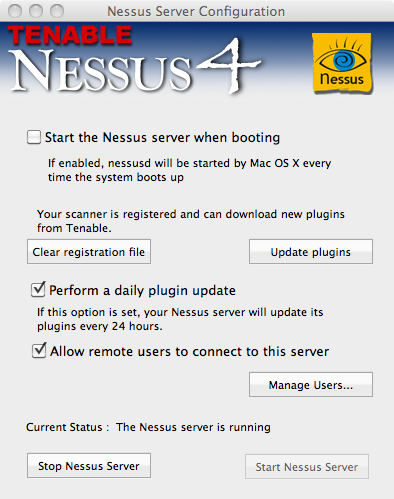
\includegraphics[width=8cm]{img/nessus_serveur.png}
	\caption{Serveur Nessus}
\end{figure}


L'application cliente Nessus que nous avons utilisé fonctionne au sein d'un navigateur. Une fois rentrée l'adresse fournie, nous arrivons sur une page 
de login. Nous nous connectons à l'aide d'un utilisateur que nous avons précédemment renseigné au sein du serveur.

\begin{figure}[H]
	\center
	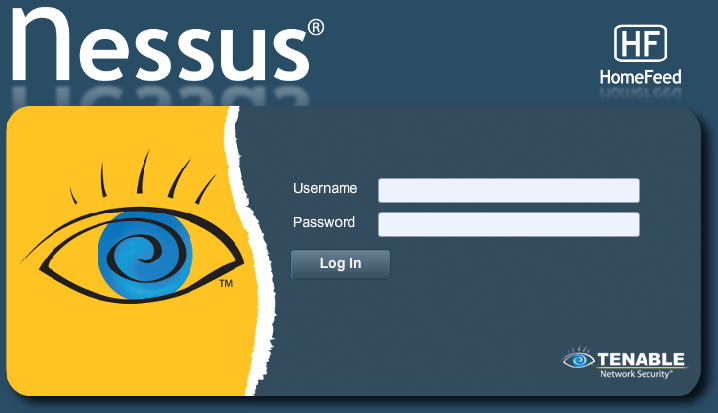
\includegraphics[width=10cm]{img/nessus_client_login.png}
	\caption{Connexion à Nessus}
\end{figure}

Suite à cette connexion, nous accédons à l'accueil permettant de gérer et utiliser Nessus.

\begin{figure}[H]
	\center
	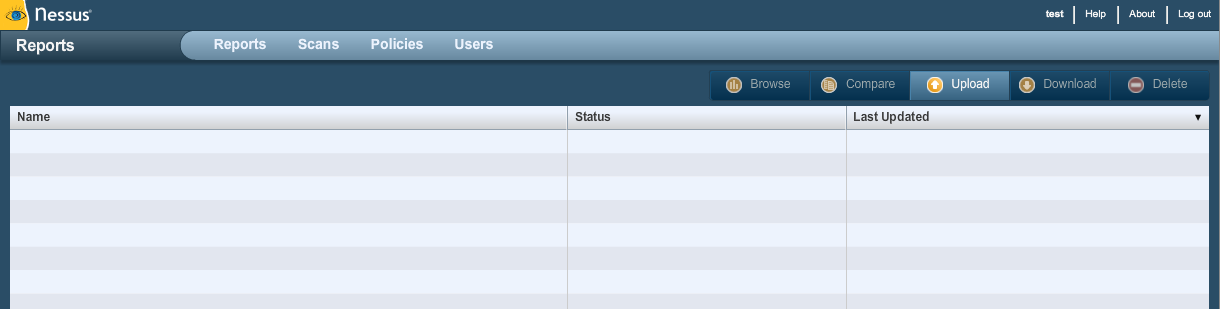
\includegraphics[width=15cm]{img/nessus_accueil.png}
	\caption{Accueil Nessus}
\end{figure}

\begin{itemize}
	\item Policy : Définition de règles (type d'attaques à effectuer, plugin à activer/désactiver, ...)
	\item Scans : Etat des scans en cours. Lors de la création d'un scan, nous lui lions une règle Policy.
	\item Reports : Contient les rapports de scans.
\end{itemize}

\subsection{Ajout d'une policy}
Dans un premier temps, nous allons créer une policy d'attaque. Celles-ci sont découpées en 4 parties :
\begin{itemize}
	\item General : Permet de définir des paramètres générales sur la règle d'attaques (nom, description, ports à scanner, ...)
	\item Credentials : Permet de définir des comptes à tester sur la cible (compte SMB, SSH, ...)
	\item Plugins : Nessus fonctionne à l'aide de plugin que l'on peut activer ou désactiver suivant la cible à attaquer. Chaque plugin correspond à une
	attaque spécifique.
	\item Preferences : Permet de fournir des informations supplémentaire (identifiant base de données, s'il faut ou non scanner du matériel fragile,...) 
\end{itemize}

Dans un premier temps, nous configurons la partie General. Nous indiquons que nous souhaitons tester tous les ports.
\begin{figure}[H]
	\center
	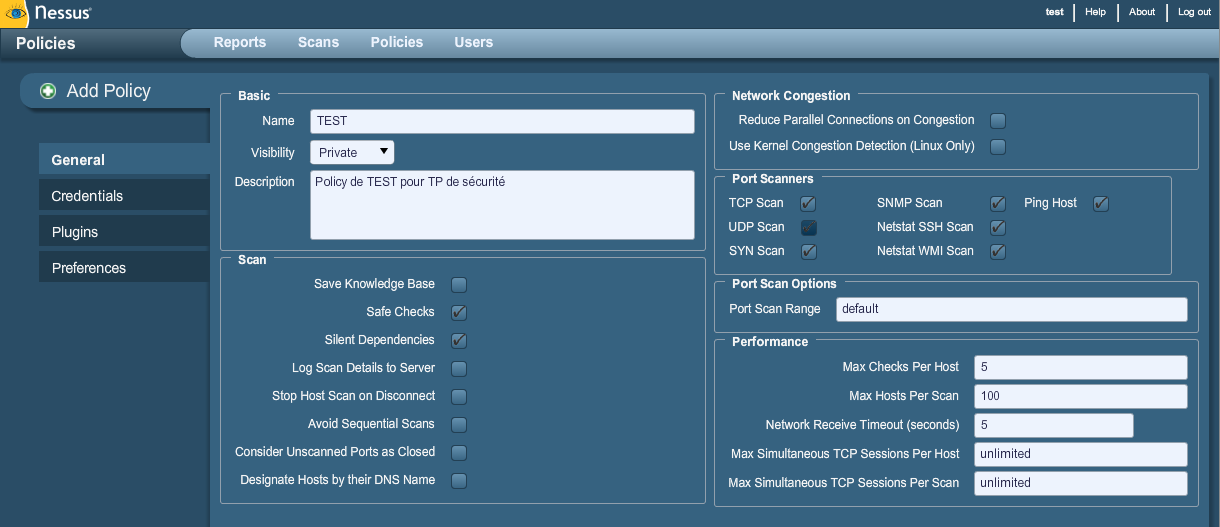
\includegraphics[width=15cm]{img/nessus_policy_general.png}
	\caption{Création d'une policy - General}
\end{figure}

Pour la partie crédentials, nous laissons les données par défaut.
\begin{figure}[H]
	\center
	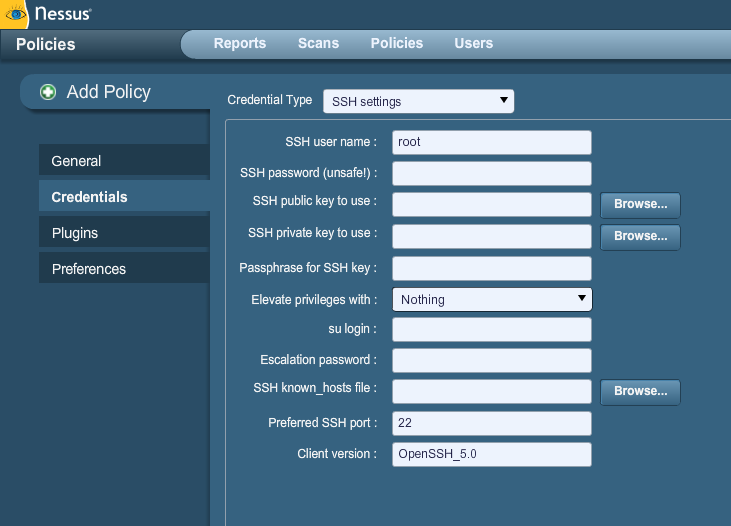
\includegraphics[width=15cm]{img/nessus_policy_credentials.png}
	\caption{Création d'une policy - Credentials}
\end{figure}

Nous ne faisons pas de restrictions au niveau des plugins et activons tout. Tous ne sont pas nécessaire en sachant que nous attaquons un ordinateur
personnel et non un serveur Apache par exemple.
\begin{figure}[H]
	\center
	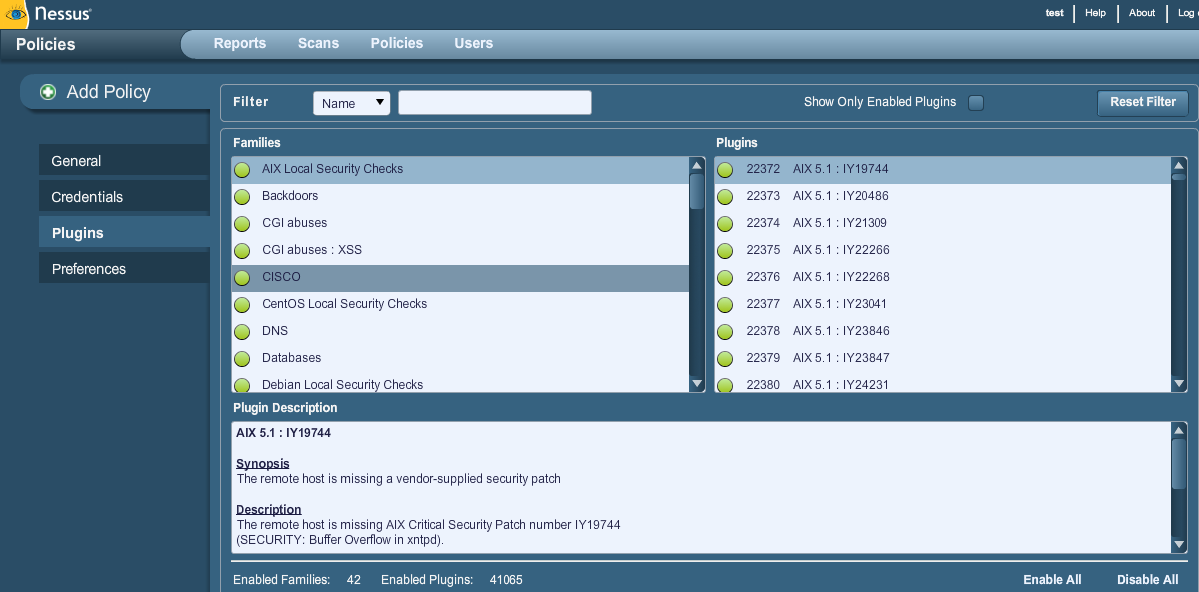
\includegraphics[width=15cm]{img/nessus_policy_plugins.png}
	\caption{Création d'une policy - Plugins}
\end{figure}

Enfin, nous laisson les préférences par défaut (pas d'utilisation de base de données, ...)
\begin{figure}[H]
	\center
	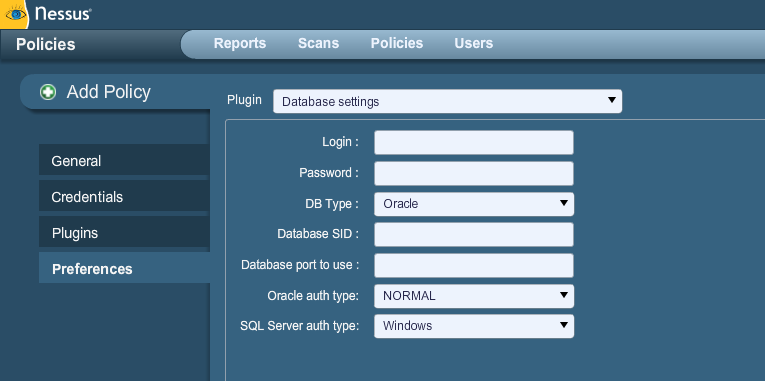
\includegraphics[width=15cm]{img/nessus_policy_preferences.png}
	\caption{Création d'une policy - Preferences}
\end{figure}

\subsection{Ajout et lancement d'un scan}
Notre policy crée, nous allons maintenant pouvoir lancer un scan l'utilisant.\\
Lors de l'ajout, nous devons renseigner un nom, la date de lancement, la policy à utiliser et, enfin, les cibles de ce scan.

\begin{figure}[H]
	\center
	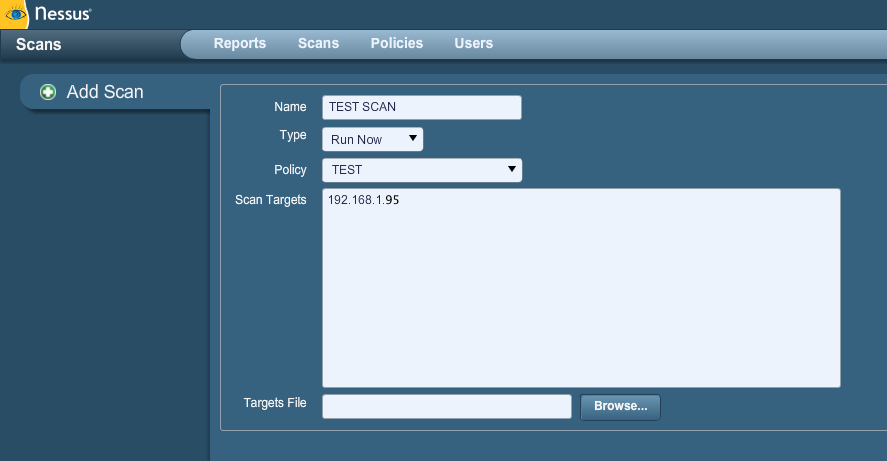
\includegraphics[width=15cm]{img/nessus_scan.png}
	\caption{Ajout d'un scan}
\end{figure}

\subsection{Résultat du scan}
Une fois le scan terminé, nous pouvons aller dans la section report afin de voir le résultat. Nous sélectionnons ainsi le scan
puis la machine cible que nous avons analysé. Les résultats sont ensuite organisé par protocole puis par port. Pour chaque protocole,
il est indiqué le nombre de failles importantes, moyennes et faibles.

\begin{figure}[H]
	\center
	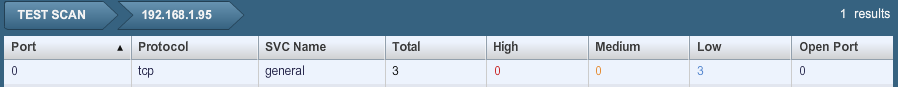
\includegraphics[width=15cm]{img/nessus_scan_protocole.png}
	\caption{Liste des protocoles possédant des failles}
\end{figure}

\begin{figure}[H]
	\center
	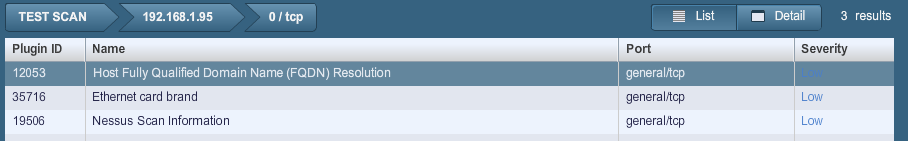
\includegraphics[width=15cm]{img/nessus_scan_tcp.png}
	\caption{Liste des failles du protocole TCP}
\end{figure}

Nous pouvons ensuite sélectionner une faille spécifique afin de voir à quoi celle-ci correspond. Pour la faille ci-dessous, Nessus indique qu'il a réussi 
à obtenir le nom complet de la cible. Dans ce cas, il n'y a aucun risque, il n'est donc pas nécessaire de prévoir quelque chose pour corriger cette faille. 
Il n'y a donc aucune solution d'indiquée.
\begin{figure}[H]
	\center
	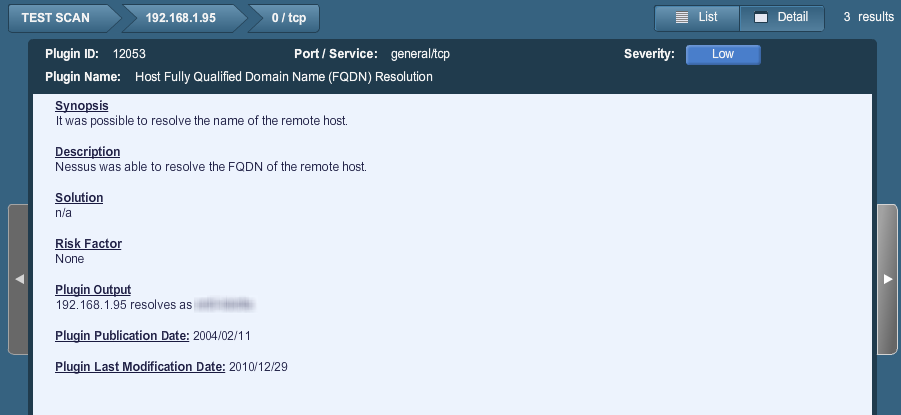
\includegraphics[width=15cm]{img/nessus_scan_faille.png}
	\caption{Précision d'une faille}
\end{figure}

Dans l'exemple ci-dessous (scan effectué sur une autre machine), on peut voir apparaître une faille important lié à l'application VMware.
Il est indiqué qu'un pirate peut utiliser différentes méthodes pour s'introduire dans le système et gagner un accès privilégier (root). On peut, cette
fois, voir apparaître une solution pour résoudre ce problème. Ici, il s'agit de simplement mettre à jour le logiciel.
\begin{figure}[H]
	\center
	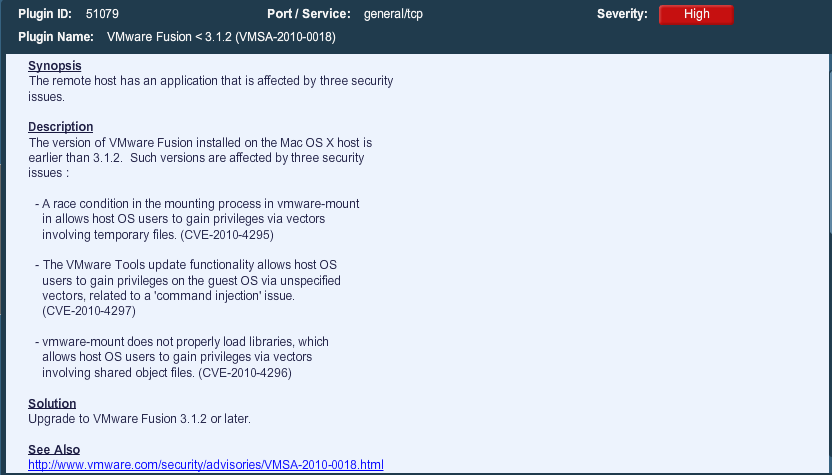
\includegraphics[width=15cm]{img/nessus_scan_vmware.png}
	\caption{Faille VMware}
\end{figure}


\subsection{snort}
Il s'agit d'un logiciel permettant de détecter les tentatives d'intrusions au sein de notre système. Pour cela, il faut définir un certain
nombre de paramètres au sein d'un fichier de configuration puis, d'indiquer les règles que nous souhaitons mettre en route (analyser HTTP, SMTP, ...).
Il a l'avantage de fournir plusieurs possibilité de log des infos (fichier texte, base de données, évènements récupérable à partir d'autres applications, ...).


\section{Analyse de fichier log}
Pour observer le contenu du fichier, nous avons utiliser Wireshark.

Suite à l'analyse du fichier log, nous avons pu déterminer que l'adresse de l'attaquant est 192.168.0.9 et celle de la cible 192.168.0.99. En effet, 
tous les paquets de demande de connexion sont envoyé de l'attaquant vers la cible.

On peut voir qu'il s'agit un scan \textit{SYN}. En effet, l'attaque effectue des demandes de connexion \textit{SYN} sur chaque port qu'il souhaite analyser.
Si la cible répond \textit{[SYN, ACK]} c'est que le port est ouvert, s'il répond \textit{[RST, ACK]} c'est qu'il ne l'ait pas.\\
Afin de connaître les ports ouverts de la cible, il ne nous fallait plus qu'à effectuer un filtre sur les paquets affichés. Une fois ceci effectué, nous avons
pu discerner que les ports SSH, SunRPC, filenet-tms, HTTP, HTTPS et DOMAIN étaient ouverts.

\newpage
\section{Annexe}
\subsection{Configuration firewall}
\lstinputlisting{img/config_reseau} 


\end{document}




